% Mid-term Paper on Concurrent Physics Engine
\documentclass[conference]{IEEEtran}

\usepackage{graphicx}
\usepackage{lettrine}
\usepackage{listings}
\usepackage{color}
\usepackage[T1]{fontenc}
\usepackage{textcomp}


\definecolor{dkgreen}{rgb}{0,0.6,0}
\definecolor{gray}{rgb}{0.5,0.5,0.5}
\definecolor{mauve}{rgb}{0.58,0,0.82}

\lstset{frame=tb,
  language=Java,
  aboveskip=3mm,
  belowskip=3mm,
  showstringspaces=false,
  columns=flexible,
  basicstyle={\small\ttfamily},
  numbers=none,
  numberstyle=\tiny\color{gray},
  keywordstyle=\color{blue},
  commentstyle=\color{dkgreen},
  stringstyle=\color{mauve},
  breaklines=true,
  breakatwhitespace=true,
  tabsize=3
}

\begin{document}

\title{A Concurrent Physics Engine}


\author{\IEEEauthorblockN{Nitish Gupta}
\IEEEauthorblockA{College of Engineering and\\Computer Science\\
University of Central Florida\\
Orlando, FL 32816\\
Email: nitesh4146@gmail.com}
\and
\IEEEauthorblockN{Sumit Bhattacharya}
\IEEEauthorblockA{College of Engineering and\\Computer Science\\
University of Central Florida\\
Orlando, FL 32816\\
Email: er.sumitbhattacharya@gmail.com}
\and
\IEEEauthorblockN{Tyler Truong}
\IEEEauthorblockA{College of Engineering and\\Computer Science\\
University of Central Florida\\
Orlando, FL 32816\\
Email: graxrabble@gmail.com}}

\maketitle

\begin{abstract}
We will compare the performance of different spatial data structures for concurrent broadphase collision detection. This includes Lists, Hash tables, and Quad Trees.
\end{abstract}

\IEEEpeerreviewmaketitle



\section{Importance of Work}

\lettrine[findent=2pt]{\textbf{T}}{ }he Broadphase Collision Detection is an important step within a physics engine which greatly impacts the performance of a physics engine. It is also the hardest part of the physics engine to parallelize. Kinematics and Collision Resolution is embarrassingly parallel: solved by dividing an array into sections and then giving each section to a thread. Brute Force Broadphase Collision detection has a runtime complexity of $O(n^2)$. Ignoring these data structures will result in a performance penalty even if all other parts of the physics engine are parallelized.


\section{Technical Overview}
We want to measure the performance of the different data structures in the context of a real time physics engine. This physics engine will move circles with random velocities around a screen. When a circle collides with the edge of the screen or another circle, it will bounce off and travel in another direction. The physics engine will divide time into equal slices called frames. The simulation will run at 60 FPS. Each frame will do the following in this order: Kinematics, Collision Detection, Collision Response. Kinematics requires add() ,remove() and update() operations as objects move around the world. Collision Detection requires a query() operation to find objects that are near each other.

Thread pooling is the basis for concurrency within the physics engine. All kinematics, collision detection and collision resolution will be divided into tasks and then submitted to the Thread pool. The threads will then take a task and execute it.

Spatial Data Structures are used by the physics engine to speed up the most intensive step, collision detection. Kinematics will update the object\textquotesingle s position and will call data structure\textquotesingle s update() operation so objects which has moved can be reindexed. The collision detection will call the data structure\textquotesingle s query() operation to get a list of possible collisions. The collisions will be verified to produce a list of all collisions. These collisions will be passed to Dynamics which will update the position and velocities of the objects.

One of the data structures we propose is a concurrent grid. Objects will be indexed into a cell within the grid. Each cell uses a list to store references to objects that are contained within the cell. Objects that border multiple cells will be stored as a reference in multiple cells. Each object will have a corresponding reference object to keep track of it\textquotesingle s current references. The reference object is required by the update() and remove() method to help it delete it\textquotesingle s old references as it moves around within the world. References are lazily deleted because it\textquotesingle s preferable to have false positives over false negatives. False positives results in an object getting collision tested even if it\textquotesingle s not colliding which will slow down the simulation. False negatives results in missing collisions which can result in objects passing through each other. The query() operation should be wait free since it is read only and it returns objects that have not been logically deleted.

\section{Technical Detail}
We have implemented concurrent versions of the SAP list [cite sap papers] and hash grid [cite ucf hash grid paper]. The implementations are tested in a physics simulation with moving objects where the data structure must detect objects that are near a point of interest.
	\subsection{Memory Management}
	Both implementation uses a simple memory pool. Nodes are allocated all at once in an array then stored in a free list. When a method needs to allocate memory, it will use CAS to pop off a node from the free list. When memory is no longer needed, it will be reinserted into the free list. The free list is designed as a stack because the order of unallocated memory does not matter and it involves no traversal. Most nodes use a counter to avoid the ABA problem. The ABA problem is made more likely due to the stack structure of the free list. It\textquotesingle s possible for a thread to deallocate then another thread to reallocate the same node quickly since that node stays at the top of the stack.
	
	\subsection{Thread pooling}
	Allocating and Reallocating threads are expensive. All concurrent functions (such as object position updates, insertions, queries, and collision detection) must be divided evenly among a set of threads. The solution is to store the functions into objects called Tasks. These tasks are passed on to the threadpool. The Tasks are stored inside of the thread pool in a linked list where worker threads can execute CAS removals to fetch the functions to execute. When a worker is done with the task node, it will return it to a free list where it can be recycled. Below is an example of a TaskNode:


\begin{lstlisting}
/*
 * Task Reference combines a counter and an index together. The counter is
 * used to solve the ABA problem.
 * - 32 bit counter
 * - 32 bit index
 *
 * note that indices start from 1 to N
 * (0 is reserved for null)
 */
typedef uint64_t TaskRef;


/*
 * Store tasks in a stack data structure
 */
class TaskNode {
    public:
    std::function<void()> task;
    TaskRef next;


    TaskNode() {
   	 task = nullptr;
   	 next = 0;
    }
};
\end{lstlisting}

The TaskNode as two main fields, task and ref. Task holds the function object which the worker threads execute. Ref stores an index and a counter. This counter is incremented every time the task is taken off the stack. This is to prevent the ABA problem. Note that task insertion is not completely nonblocking. It\textquotesingle s possible to block if the free list is empty.

	\subsection{SAP Implementation}
	A doubly linked list is used to store the positions of the simulation objects. It has a position and a width field. These two values are used to construct a line segment along the axis which will be used to collision test with other line segments. A third field called EID stores the ID of the Entity that the node represents. This is so the SAP algorithm can detect which objects are intersecting. This information will be passed onto other parts of the simulation.


The interesting concurrency related fields is the SapRef which is shown below. The reference field stores: an index to the previous node, an index to the next node, an ABA counter, a logical deletion bit. All of that information must be stored within a single field so CAS can atomically update them all at once.

\begin{lstlisting}
/*
 * SapRef is a bitfield that stores all pointers, counter, flag data in a
 * single bitfield
 *
 * - 20 bit prev
 * - 20 bit next
 * - 23 bit reference counter
 * - 1 bit marked
 */
typedef uint64_t SapRef;

/*
 * Node which store the ID, position, and width of an object.
 */
class SapNodeLF {
    public:
    SapNodeLF() {
   	 eid = 0;
   	 position = 0.0f;
   	 width = 0.0f;
   	 ref = 0;
    };

    // reference to the object that this node represents
    int eid;

    // position along the axis
    float position;

    // size of the object
    float width;

    // reference field which contains both prev and next pointers
    std::atomic<SapRef> ref;
};

\end{lstlisting}

Note that this list has both a previous and a next field. This is a doubly linked list. The double linking helps boost performance by avoiding the need to traverse from the head of the list to reach a previous value (which is common in a physics simulation). One problem is that it\textquotesingle s impossible to insert a node into a doubly linked list atomically without a Double CAS. One solution mentioned in a research paper by [Haken] is to treat the previous pointer as only a hint.\\

Insertion Algorithm:
\begin{enumerate}
\item Node.prev -> predecessor
\item Node.next -> successor
\item Predecessor.next -> Node
\item Successor.prev -> Node
\end{enumerate} 


The insertion algorithm linearizes at step 3 where the node first becomes accessible to the list. This makes the list a valid singly linked list in the forward direction. Even if the Successor doesn\textquotesingle t point to the node directly (Successor.prev still points to Predecessor), it is still accessible though the Predecessor\textquotesingle s next pointer. All prev pointers will point to a location somewhere behind them. To reach a node with a lesser value somewhere behind the current node, follow the prev pointers until the target node has a larger value, then follow the next pointers.


Deletion Algorithm:
\begin{enumerate}
\item Node.marked = True
\item Predecessor.next -> Successor
\item Successor.prev -> Predecessor
\item ReferenceCount Until Garbage Collection
\end{enumerate} 

Deletion is very similar to deleting a node from a singly linked list with one exception. Deletion is more ugly because any node in the list is allowed to reference any arbitrary node behind it. Even if the predecessor and successor no longer references the current node, any node ahead of the list could possibly reference the current node. Deleting the node while it  can still referenced by a stray previous pointer will have disastrous consequences. Reference Counting is needed to tell when no more nodes are pointing to the current node which means it is safe to delete. We tried to ignore this step with an ABA counter which resulted in disastrous results.

	\subsection{Hash Grid Data Structure}
	The grid data structure subdivides floating point space into integer coordinates. These coordinates are then mapped into buckets with a hash function. The current hash function simply wraps around the edge of the data structure (nothing fancy). The main concurrency problems with the Hash Grid is needing linked lists to support all of the internal references.

\begin{lstlisting}	
/*
     * Hash function which maps x, y coordinates into a bucket.
     * Currently is a 10 x 10 grid which wraps around at the edges.
     */
    void hash_func(int &row, int &col, float x, float y) {
   	 col = std::rint((x / cell_size) - 0.5f);
   	 row = std::rint((y / cell_size) - 0.5f);
    };
    // hash integer coordinates to bucket
    auto hash = (j % 100) + 100 * (i % 100);
    auto &bucket = buckets[hash];
\end{lstlisting}

The hash buckets store objects by chaining them in a linked list. Each linked list is treated as a concurrent stack which uses CAS insertion and removals. FILO is used because the order of the data within the buckets do not matter since they all must be traversed anyway. Each bucket will hold a linked list which points to every object.

Each object must know which buckets it occupies so it can check for its neighbors. Since each object is able to occupy multiple buckets at once, it must also store a linked list which points to the buckets in the hash table. Both of these linked lists must be updated every time an object moves.

A third and final linked list is temporarily created by the query function. It\textquotesingle s possible for objects to collide with each other multiple times in different buckets. This is incorrect since two objects cannot collide with each other multiple times simultaneously; they can only collide once. If object A is in buckets [1, 2, 3] and object B is in buckets [2, 3, 4]; they will collide twice at buckets [2, 3]. A linked list is needed to keep track of previously detected collisions to avoid multiple collisions.

All of the linked lists share the same GridNode class. All of the GridNodes are stored within a single memory pool for simplicity. Anytime a node needs to be allocated, it can pop a new node off the free list within the Grid. It\textquotesingle s possible for the Grid to block if the free list is empty.

\section{Evaluation}
SAP Algorithm works well for small number of objects. It performs better than the Grid for double digit number of objects. This is not surprising since Grid has a lot of overhead; lots of internal linked lists, allocations, memory pool. A deviation can be noticed at around 500 objects. This trend grows stronger until the number of objects reach 5000. At this large number, the O(n log n) runtime complexity of SAP reveals itself. Notice how the runtime of grid increases proportionally with the number of objects, showing it\textquotesingle s O(n) runtime complexity.

\begin{figure}[!h]
\centering
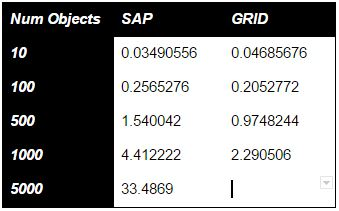
\includegraphics[scale=0.9]{table1}
\caption{Chart 1}
\label{fig_sim}
\end{figure}

\begin{figure}[!h]
\centering
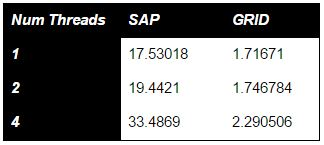
\includegraphics[scale=0.9]{table2}
\caption{Chart 2}
\label{fig_sim}
\end{figure}


This Second Chart shows that Both of these algorithms failed to increase performance as the number of threads increases. This is most likely caused by contention. The increase of contention is modest from 1 to 2 threads. The contention in SAP increases by 72 percent between 2 and 4 threads. That\textquotesingle s most likely because the threads must compete for CAS on references spread out along the entire list. This is probably caused by tasks being issued near each other. We issued tasks in order for simplicity. There could be room for improvement if we issued tasks randomly which can help spread out the contention.

Note that as the number of threads increases, the time it takes to complete gets longer. This means that multithreading our implementation made things worse.



\section{Conclusion}
We tested how contention affects list and grid based data structures for concurrent spatial data structures. Making programs fast requires more than slapping on an atomic here and there. Our concurrent data structures performed worse as the number of threads increased. This is because of naive design decisions such as making the free list and memory pool a simple stack.

\begin{figure}[!h]
\centering
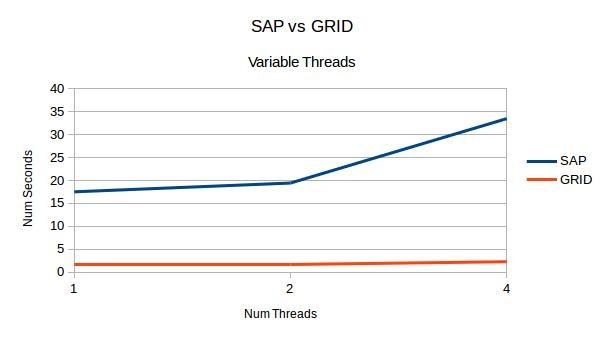
\includegraphics[scale=0.5]{sap_grid}
\caption{Sap vs Grid}
\label{fig_sim}
\end{figure}

\begin{figure}[!h]
\centering
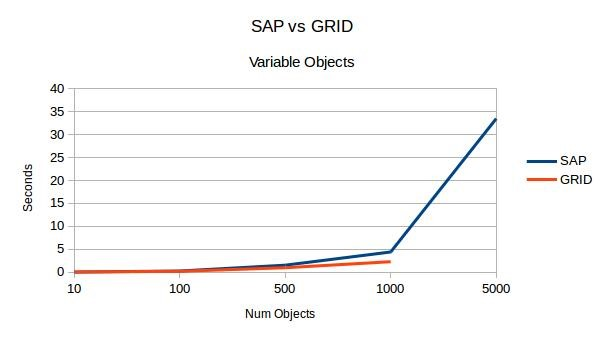
\includegraphics[scale=0.5]{sap_grid2}
\caption{Sap vs Grid}
\label{fig_sim}
\end{figure}

\section{Related Work}
There are few works based on concurrent spatial data structures. Most of the literature on spatial data structures was written before lock free programming. The exception is the QuadBoost QuadTree paper which was published in June of 2016, 4 months ago. The paper starts by mentioning a basic CAS QuadTree implementation. Because a quadtree has four children, all of their pointers cannot be changed atomically. This is solved with a flag which locks the node. Another problem mentioned in the paper is lazy deletion. Lazy deletion causes the tree to grow too large; objects will move around the world, forcing the quadtree to add and delete many nodes. When a node has no more objects, it becomes empty. Those empty nodes which are lazy deleted consumes lots of memory. One solution the authors found was to use state transitions to keep track of how many empty nodes are on a branch and then force a compress operation on that branch when it\textquotesingle s full of empty nodes. The compress operation will pull objects up to parent instead of leaving leaving them in the chain of empty nodes. This will allow the tree to free up old memory.

\section{Appendix}
	\subsection{Physics Engine}
	Physics Engine is a class or library which handles motions and collisions of a set of objects. Motion and collision are usually handled with Kinematics and Dynamics equations. Videogames are an example of programs that use physics engines. The video game will tell the engine to keep track of all players and projectiles. The engine will report to the video game when a projectile hits a player or when a player walks into a wall. This allows the programmer to focus on other tasks like Graphics or AI.

	\subsubsection{Collision Detection}
	Collision Detection is the process of detecting collisions between objects. Imagine two circles traveling towards each other in a head on collision. The physics engine must detect the exact time $t$ when the two circles collide and then their new velocities after the collision. Physics engine literature commonly splits collision detection into two steps: narrowphase and broadphase.

\begin{figure}[!h]
\centering
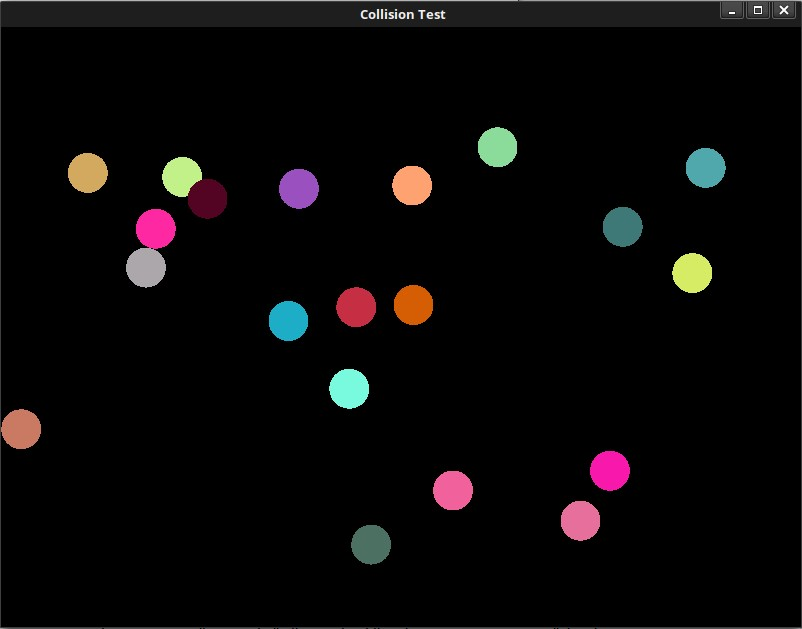
\includegraphics[scale=0.27]{collision}
\caption{Box2D implementation}
\label{fig_sim}
\end{figure}

	\subsubsection{Narrowphase}
	Narrowphase focuses on detecting the TOI of a collision between two objects. The two objects are then backtracked to a previous position so they stop intersecting with each other. A new velocity or trajectory is then computed using Collision Resolution.
	\subsubsection{Brute Force}
	Brute Force Collision Detection has a runtime complexity of $O(n^2)$. This is because the set of all collisions is a permutation of every pair of N objects. 

\begin{figure}[!h]
\centering
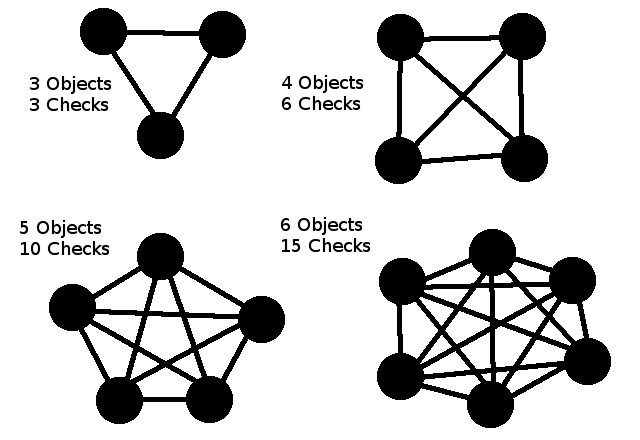
\includegraphics[scale=0.4]{brute}
\caption{Brute Force Collision Detection}
\label{fig_sim}
\end{figure}
	
	This runtime is not noticeable with 100 objects but is very noticeable with 1000 objects. Even though the number of jects increased by 10 folds, the runtime complexity increased by 100 folds.
	\subsubsection{Broadphase}
	Broadphase Collision Detection is used to accelerate Collision Detection by sorting objects into spatial data structures: Lists, Hash tables, and Quad Trees. Objects are sorted by their position within the world. All of the above data structures take advantage of the fact that only objects that are nearest to each other need to be checked for collision.

	\subsection{Lists}
	Lists are the simplest spatial data structures. Imagine two objects on a number line. The numbers 2 and 4 are closer to each other than 2 and 24, so the numbers 2 and 4 are more likely to collide with each other compared to 2 and 24. Lists are used by the SAP or Sweep And Prune algorithm which is based on the converse of the SAT or Separating Axis Theorem. SAT states that objects can only collide if they intersect on all axises. The converse is that objects cannot collide if they do not intersect on one of many axis. This number line will be referred to as the chosen axis. SAP works by checking for collisions between pairs of objects that are near each other on the chosen axis; this is the Sweep step. SAP will check the proximity of objects near a query point on the chosen axis. If an object does not intersect with the query point then the object will not collide; this is the Prune step. The remaining pairs that were not pruned could collide and will be passed to either another layer of SAP on a different axis or to the narrowphase collision detection.\\

\begin{figure}[!h]
\centering
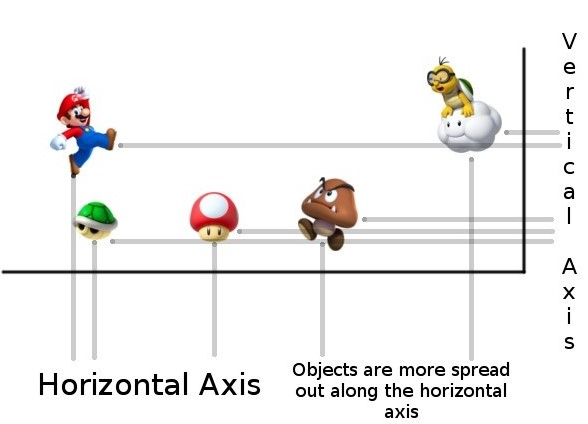
\includegraphics[scale=0.4]{sweep}
\caption{Sweep and Prune: Axis Comparison}
\label{fig_sim}
\end{figure}

\begin{itemize}
  \item Advantages of Lists:\\
  Lists are the simplest data structures to implement. This also means they are the easiest data structure to parallelize. The data structure will focus on implementing the swap() operation over the add() and delete() operations. Imagine a 2d world with two balls named A and B. A is located on the left while B is located on the right. These two balls are moving towards each other along the horizontal axis which is also the chosen axis for SAP. Note that it is possible for A and B to not collide if they have different heights within the 2d world. By not colliding they will pass through each other and swap positions along the chosen axis. Now, it is B that is located on the left while A is located on the right. Instead of deleting nodes and adding nodes to the List, they can be swapped. The swap operation() avoids garbage collection of the nodes.\\
  
  \item Disadvantages of Lists:\\
  They check for collisions on a single axis. The algorithm will break down if the objects do not spread out along the chosen axis. Imagine Super Mario World which has Mario and all of the enemies on running along platforms at different heights. The SAP will fail if the vertical axis is chosen because most of the objects will cluster along the same height. A better axis would be the horizontal axis because all of the objects on the screen will be spread out more. One solution is to calculate the standard deviation along multiple axis and choose the one with the largest deviation.
\end{itemize}

	\subsection{Grids}
	Grid data structure: imagine one airplane in New York and another airplane in California. The two airplanes are so far apart that checking for collision is not necessary. The 50 states within America act as the grid. Airplanes can only collide with each other in two cases: both planes are within the same state and both planes are near the borders between neighboring states. Grids are normally composed of square cells for ease of implementation. The Grid data structure works by mapping all objects into cells. This speeds up collision detection because each cell divides Broadphase Collision Detection into series of small Brute Force Collision Detections.\\
	
\begin{figure}[!h]
\centering
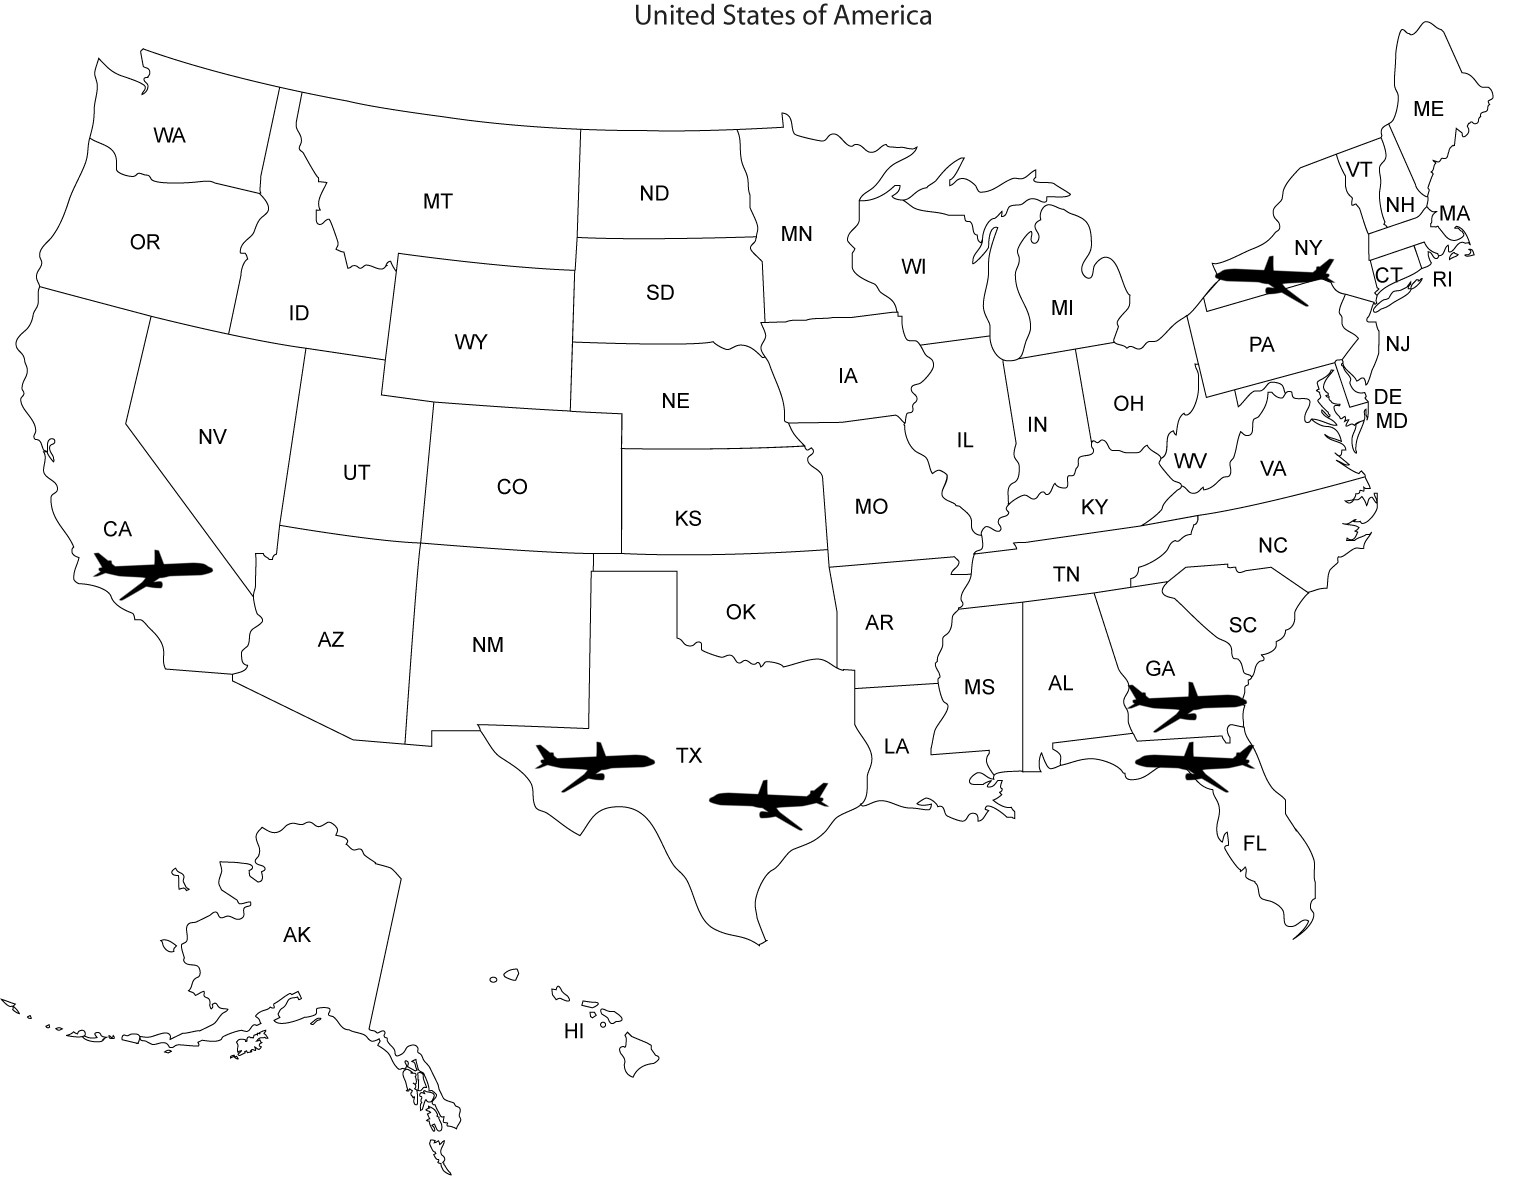
\includegraphics[scale=0.15]{usa}
\caption{Grid Analogy}
\label{fig_sim}
\end{figure}

\begin{itemize}
  \item Advantages of Grids:\\
  Grids are the most efficient data structure for sparse, uniformly distributed, and homogeneous objects. Imagine 100 circles of the same size spaced in a lattice pattern across the world where each circle has it\textquotesingle s own cell. The Query() operation works by returning all other objects within the same and neighboring cells. The add() and remove() operation can be implemented as a lookup table of lists where each cell is represented by a list. The list data structure can easily be parallelized by lock free techniques. And the lookup table can distribute threads across the data structure, reducing contention.\\
  \item Disadvantages of Grids:\\
  Grids degrade when objects are not sparse, uniform and homogenous. The worse case is where all objects are clustered into same cell. This Grid will degrade into Brute Force collision detection. When an object is larger than a single cell of the Grid, the Grid must store that object into multiple cells. This means that the grid must perform multiple add() and remove() operations for every cell that contains the large object. The Grid must also handle objects that are on the border between multiple cells. There are two solutions: store the object into multiple cells similar to the large object problem or store the object in one cell and the query() operation will check neighboring cells.
\end{itemize}

	\subsection{Quadtrees}
	Quadtrees are similar to the grid based data structures with one added feature. They recursively subdivide the space of all objects into quadrants. This means that every node in the tree will have four children, one for each quadrant. The tree gives this spatial data structure a runtime complexity of $O(\log{n})$ because each traversal in the tree will prune $3/4^{th}$ of the possible collisions.\\

\begin{figure}[!h]
\centering
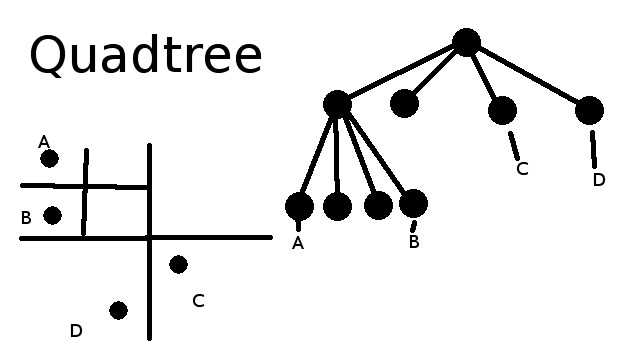
\includegraphics[scale=0.38]{quadtree}
\caption{A Quadtree}
\label{fig_sim}
\end{figure}
	
\begin{itemize}
  \item Advantages of Quadtrees:\\
  Quadtrees can recursively divide space into smaller chunks. They can efficiently handle objects of different sizes. Grids store large objects in multiple cells while Quadtrees can subdivide cells until they fit around the object. Quadtrees are less vulnerable than Grids to objects clustering near each other. Where the Grid degenerated into Brute Force Collision Detection, the Quadtree can subdivide cells.\\
  \item Disadvantages of Quadtrees:\\
  Quadtrees are more complicated to implement because they involve creating and deleting nodes. This means that new problems such as memory management, garbage collection and ABA must be considered. The Quadtree will constantly change shape as objects move around in the world. Imagine a racing game where cars move around a track. The track will be subdivided into quadrants which are recursively subdivided until fitting the nodes fit the cars. When the cars move from the top right corner to the top left corner, all of the tree structure must be deleted from the top right quadrant and recreated on the top right quadrant.\\
\end{itemize}

	\subsection{Collision Resolution}
	Collision Resolution is the process of calculating an object\textquotesingle s new velocity after a collision. The programmer has full artistic freedom to decide how objects should behave. An example of a parameter is elasticity or the bounciness of an object: a rubber ball should bounce of the ground while a sandbag will stick to the ground. Another parameter is mass: lighter objects should experience a greater change in velocity when bouncing off a heavier object. Resolution is not a focus of this paper, so a simple reflection is used to compute the new velocities of objects.\\
	
	\subsection{Thread Pooling}
	Thread Pooling is a technique which creates a set number of threads then delegating tasks to the threads. Initializing and Destroying threads is expensive which is why a pool of threads are kept alive. It works by dividing computation into a unit called a task. A task can be checking if a pair of objects are colliding. A FIFO concurrent queue is used to store the tasks. Available threads will fetch the tasks from the queue then execute each task. This provides load balancing between the threads.
	

\begin{thebibliography}{}

\bibitem{quadboost}
K.~Zhou, G.~Tan and W.~Zhou, \emph{Quadboost: A Scalable Concurrent Quadtree}.

\bibitem{rtrees}
M.~Kornacker and D.~Banks, \emph{High-Concurrency Locking in R-Trees}.

\bibitem{hashing}
E.~Hastings, J.~Mesit and R.~Guha, \emph{Optimization of Large-Scale, Real-Time Simulations by Spatial Hashing}.

\bibitem{pcollision}
Y.~Serpa and M.~Rodrigues, \emph{Parallelizing Broad Phase Collision Detection for Animation in
Games: A Performance Comparison of CPU and GPU Algorithms}.

\bibitem{sweepprune}
D.~Tracy, S.~Buss and B.~Woods, \emph{Efficient Large-Scale Sweep and Prune Methods with AABB Insertion and
Removal}.

\bibitem{treemaster}
Joshua Shagam, \emph{Dynamic Spatial Partitioning for Real-Time Visibility Determination}.

\bibitem{kinetic}
D.~Coming and O.~Staadt, \emph{Kinetic Sweep and Prune for Collision Detection}.

\bibitem{kinetic}
Hakan Sundell and Philippas Tsigas, \emph{Lock-Free and Practical Doubly Linked List-Based Deques Using Single-Word Compare-and-Swap}.
\end{thebibliography}

\end{document}